\section{Entwicklungsumgebung}
Da nun die zu verwendenden Technologien und Tools gewählt sind, kann mit der
eigentlichen Entwicklung des Prototypen begonnen werden. Als erster Schritt
muss die Entwicklungsumgebung gewählt und eingerichtet werden.

\subsection{Betriebssystem}
Privat und in meiner Firma arbeite ich mit dem Betriebssystem ``MacOS X'' von ``Apple'',
welches sich auch sehr gut für die Entwicklung von `Ruby on Rails' Webapplikationen
eignet, da ``Apple'' seit Version 10.4.6 von ``MacOS X'' `Ruby' und `Ruby on Rails' 
mitliefert \cite{macosx}.

Ich werde den Prototypen mit ``MacOS X'' Version 10.6.5 erstellen.

\subsection{Integrierte Entwicklungsumgebung}
Wenn man zum Beispiel eine Applikation mit `Java' entwickelt, wird sehr oft eine
sogenannte ``Integrierte Entwicklungsumgebung'' \cite{ide}, kurz `IDE', verwendet.
Diese bieten meist einen Texteditor, Compiler bzw. Interpreter, Linker, Debugger
und viele Quelltextformatierungsfunktionen.

Für die Entwicklung von `Ruby on Rails' Applikationen hat sich auf ``MacOS X''
jedoch schon sehr früh ein relativ einfacher und doch sehr guter Texteditor
namens ``Textmate'' durchgesetzt. Er wurde von Anfang an in den offiziellen Videotutorials 
von `rubyonrails.org' verwendet und auch Ryan Bates, eine Koryphäe in der
`Ruby on Rails' Welt, arbeitet ausschliesslich damit \cite{ryanbates}. 

Hinzu kommt ``Terminal'', das Kommandozeilen-Programm von ``MacOS X'', mit
dem man den lokalen Webserver startet, diverse `Ruby on Rails' Skripte ausführt
und auch `Git', das Versionsverwaltungssystem, bedient.

Ich arbeite, um den Prototypen zu erstellen, mit ``Textmate'' Version 1.5.10
und dem ``Terminal'' Version 2.1.1.

\subsection{Versionsverwaltungssystem}
Ich habe mich entschlossen mit `Git' zu arbeiten und den Quellcode auf ``GitHub''
zur Verfügung zu stellen. Für den Prototypen möchte ich mit dem 
``Standard Branching Model'' \cite{branching_model} arbeiten. Das bedeutet, dass ich
zwei der sogenannte Äste (``Branches'') führe. Einen für die Entwicklung namens 
`develop' und einen für die produktive Version namens `master'.

Wie dieses Modell funktioniert, wird in der Grafik \ref{branching_model} gut erklärt.
 
\begin{figure}[ht]
    \begin{center}
        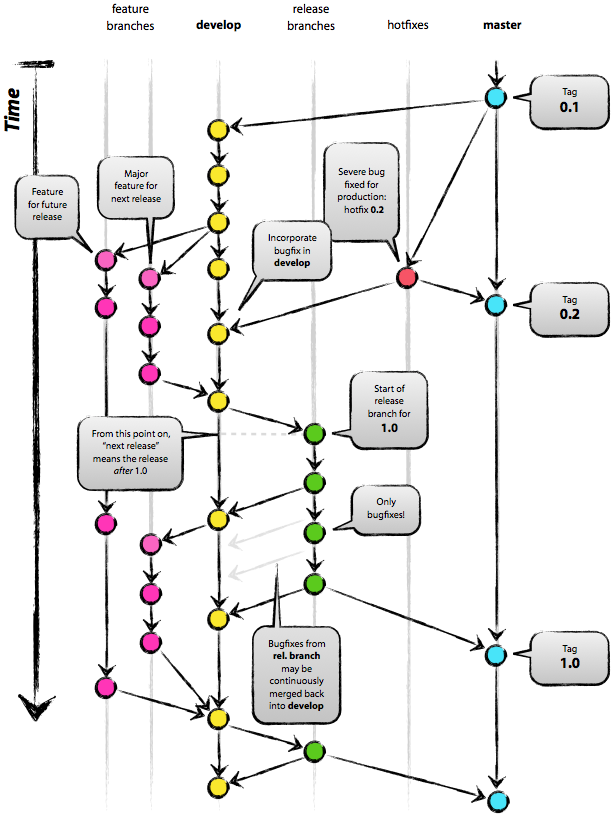
\includegraphics[width=1\textwidth,angle=0]{./bilder/branching_model.png}
        \caption{``A successful Git branching model'' von Vincent Driessen}
        \label{branching_model}
    \end{center}
\end{figure}

\clearpage

Ich habe hierzu einen privaten Account auf ``GitHub'' erstellt, welcher unter
\url{https://github.com/sspross} zu finden ist. Dieses Projekt ``OpenMediaLibrary''
habe ich unter \url{https://github.com/sspross/oml} eröffnet und öffentlich
verfügbar gemacht.

Wie das vorher erwähnte ``Branching Model'' dann in der Praxis aussieht, kann 
man auf der Grafik \ref{network_01} sehen.

\begin{figure}[ht]
    \begin{center}
        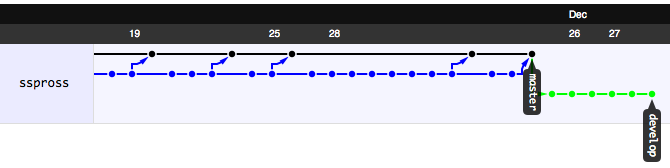
\includegraphics[width=0.8\textwidth,angle=0]{./bilder/network_01.png}
        \caption{Branches in der Praxis auf ``GitHub''}
        \label{network_01}
    \end{center}
\end{figure}

Die schwarze Linie ist der `master' Branch. Jeder schwarze Punkt widerspiegelt
einen produktiven Release, der in sich abgeschlossen ist und stabil läuft.

Die blaue Linie ist der `develop' Branch und jeder blaue Punkt stellt einen
Entwicklungsschritt dar, der jedoch nicht zwingend lauffähig, aber kompilierbar 
sein muss. Die grüne Linie ist ebenfalls der `develop' Branch und dient nur
der besseren Darstellung, bis er wieder in den `master' zurückgeführt wird.

Der vollständige und immer aktuelle Verlauf der Branches kann unter 
\url{https://github.com/sspross/oml/network} jederzeit eingesehen werden.

\section{Umsetzung}
Ich möchte in diesem Kapitel nicht auf die ganze Entstehung des Quellcodes 
eingehen, da dieser und dessen Verlauf vollständig auf ``GitHub'' unter
\url{https://github.com/sspross/oml} einsehbar ist.

Jedoch erläutere ich, welche Zusatzsoftware, auch genannt ``Plugins'' \cite{plugin}, ich 
verwendet habe und weshalb. Zusätzlich gehe ich auf grössere Herausforderungen,
die sich mir während der Entwicklung gestellt haben, ein und wie ich sie
gemeistert habe.

\subsection{Zusatzsoftware}
In der nachstehenden Tabelle \ref{tab:plugins} liste ich die zusätzlich verwendeten
``Software'', geschrieben für das Framework `Ruby on Rails', auf und erläutere
ihren Verwendungszweck. Die Versionen sind als kurzer Hash \cite{hash} des
jeweiligen Projektes auf ``GitHub'' angegeben.

\begin{table}[ht]
\begin{center}
    \begin{tabular}{llp{6cm}lp{3cm}}
        \toprule Nr & Plugin & Verwendungszweck & Version & Herkunft \\
        \midrule 1 & project zero & Ein leeres `Ruby on Rails' 3.0 Template, welches
                 schon vorkonfigurierte Authentifizierungs-, Templating- und Testingfunktionen
                 mitliefert. & 8fb458c & \url{https://github.com/panter/project_zero} \\
        \midrule 2 & globalize3 & Bietet die Möglichkeit einfacher Objektinstanzen
                 zu internationalisieren. & aecb42f & \url{https://github.com/svenfuchs/globalize3} \\
        \midrule 3 & factory girl rails & Damit können Factories \cite{factory} für Tests
                 erstellt werden. & 5448687 & \url{https://github.com/thoughtbot/factory_girl_rails} \\
        \midrule 4 & resource controller & Hilft die Standard RESTful \cite{restful} Controller mit weniger Code
                 zu implementieren. & 48359da & \url{https://github.com/jamesgolick/resource_controller} \\
        \bottomrule
    \end{tabular}
    \caption{Verwendete ``Plugins'' und deren Verwendungszweck}
    \label{tab:plugins}
\end{center}
\end{table}

\clearpage

\subsection{Herausforderungen}\label{chp:herausforderungen}
\subsubsection{Ruby on Rails Versionen}
Als ich begann den Prototypen zu entwickeln, verwendete ich die damals aktuelle
`Ruby on Rails' Version 2.3.4. Während der Weiterentwicklung gab es mehrere
Aktualisierungen von `Ruby on Rails' und ich musste auf die Version 2.3.8
updaten. Dies war kein Problem, da es sich dabei hauptsächlich um interne
Veränderungen von `Ruby on Rails' handelte, die nur einen minimalen Einfluss 
auf meinen bestehenden Quellcode hatten.

Gegen Mitte der Entwicklung erschien die `Ruby on Rails' Version 3.0 und wie
an der Versionsnummer schon zu erkennen ist, wurden darin grundlegende Dinge
verändert und verbessert. Da ich den Anspruch erhebe, einen Prototypen zu schreiben,
der auch von Drittentwicklern weiterentwickelt werden kann, musste ich meiner
Meinung nach zwingend auf die neue Version updaten, damit die Wahrscheinlichkeit
höher ist, zusätzliche Entwickler zu motivieren.

Dies stellte sich als nicht ganz einfach heraus. Als erstes versuchte ich
den bestehenden Quellcode, wie in den voran gegangenen Versionen, einfach anzupassen.
Dies reichte jedoch nicht und endete in einer Sackgasse, die sich in meinem
Quellcode als eigener Branch widerspiegelt, der nicht wieder in den `develop'
Branch zurückgeführt wurde. Dies kann man aus der Grafik \ref{deadend} entnehmen.

\begin{figure}[ht]
    \begin{center}
        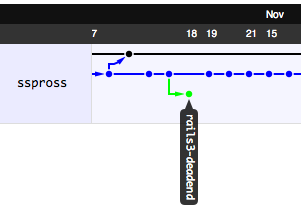
\includegraphics[width=0.3\textwidth,angle=0]{./bilder/deadend.png}
        \caption{Nicht zurückgeführter Branch `rails3-deadend'}
        \label{deadend}
    \end{center}
\end{figure}

Danach blieb mir nichts anderes übrig als den Quellcode nochmals neu auf einer
leeren `Ruby on Rails' 3.0 Instanz aufzubauen. Jedoch war es am Ende nur halb
so aufwändig, da sich in den Grundsätzen von `Ruby on Rails' nichts geändert 
hatte und somit der bestehende Code mehr oder weniger kopiert werden konnte.

Dazu hatte ich natürlich einen weiteren Branch namens `rails3' erstellt, der
dann wieder in den `develop' Branch zurückgeführt werden konnte, wie man
auf der Grafik \ref{rails3} erkennen kann.

\begin{figure}[ht]
    \begin{center}
        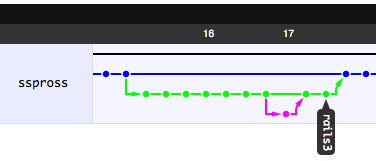
\includegraphics[width=0.4\textwidth,angle=0]{./bilder/rails3.png}
        \caption{Erfolgreich zurückgeführter Branch `rails3'}
        \label{rails3}
    \end{center}
\end{figure}

\clearpage

\subsubsection{Deplyoment}
Beim Deployment, auch ``Softwareverteilung'' \cite{deployment} genannt, stellte 
sich mir das Problem, dass ich lokal mit einer `SQlite' Datenbank entwickelt habe
und in der Produktion, also auf dem Zielserver, wo dann der Prototyp installiert
wird, mit einer `mySQL' Datenbank arbeiten wollte.

`Ruby on Rails' unterstützt von Haus aus mehrere verschiedene Datenbanktypen und
ist fähig mit `SQlite' und `mySQL' umzugehen. Jedoch ist `mySQL' abhängig vom
System, auf welchem es installiert wird.

Es war sehr viel Recherche nötig, aber am Schluss konnte ich, unteranderem mit
der Hilfe meines Betreuers, `mySQL' bei der Installation explizit deaktivieren,
damit auf dem Zielserver nicht versucht wird, eine weiter `mySQL' Instanz zu
installieren. Zusätzlich konnte ich im sogenannten `Gemfile' elegant festlegen,
in welcher Umgebung welcher Datenbankadapter verwendet werden soll:

\begin{verbatim}
    group :development, :test do
      gem 'sqlite3-ruby'
    end
    
    group :production do
      gem 'mysql'
    end
\end{verbatim}

Dadurch wird definiert, dass bei einer lokalen Installation für die Entwicklungs-
(``Development'') und für die Testumgebung der `sqlite' Adapter und in der 
Produktionsumgebung (``Production'') der `mysql' Adapter verwendet wird.

\section{Testen}
\subsection{Testfälle}
Meine Testfälle ergeben sich aus den Muss-Funktionen aus Kapitel~\ref{chp:muss_funktionen}
und sind in der nachstehenden Tabelle \ref{tab:testfaelle} mit einer klaren Frage
ausformuliert, die dann getestet werden kann.

\begin{table}[ht]
\begin{center}
    \begin{tabular}{llp{10cm}}
        \toprule Nr & Muss-Funktion & Testfrage \\
        \midrule 1 & 1 & Kann sich ein neuer Benutzer mit einem Benutzernamen und
                 einem Passwort registrieren? \\
        \midrule 2 & 1 & Kann ein Benutzernamen nur einmal verwendet werden? \\
        \midrule 3 & 2 & Kann sich der Benutzer mit seinem Benutzernamen und
                 Passwort anmelden? \\
        \midrule 4 & 3 & Kann ein neuer Film erfasst werden? \\
        \midrule 5 & 3 & Kann ein bestehender Film bearbeitet werden? \\
        \midrule 6 & 3 & Kann ein bestehender Film gelöscht werden? \\
        \midrule 7 & 4 & Kann die normale Bewertung eines Filmes von allen
                 Besuchern betrachtet werden? \\
        \midrule 8 & 5 & Kann ein angemeldeter Benutzer einen Film mit Kommentar
                 bewerten? \\
        \midrule 9 & 6 & Kann ein angemeldeter Benutzer die Bewertung über
                 seinen Freundeskreis sehen? \\
        \midrule 10 & 7 & Sind die statischen und dynamischen Inhalte in
                 mehreren Sprachen verfügbar? \\
        \midrule 11 & 8 & Kann über die API ein Film erfasst werden? \\
        \midrule 12 & 8 & Kann über die API ein Film bearbeitet werden? \\
        \midrule 13 & 8 & Kann über die API ein Film gelöscht werden? \\
        \midrule 14 & 8 & Kann die Bewertung eines Filmes über die API
                 betrachtet werden? \\
        \bottomrule
    \end{tabular}
    \caption{Testfälle basierend auf denn Muss-Funktionen}
    \label{tab:testfaelle}
\end{center}
\end{table}

\clearpage

Ich teste nun die definierten Testfälle auf meiner lokalen Instanz des 
Prototypen, der über \url{http://localhost:3000/} erreichbar ist.

\subsubsection{Registrierung}
Um die Registrierung zu testen, rufe ich den Registrierungsscreen auf und fülle
den Benutzernamen, das Passwort und die Passwortwiederholung aus und drücke dann auf
`Register'. Den Registrierungsscreen sieht man in der Grafik \ref{test_registrierung_01}
und die Bestätigung der Registrierung in der Grafik \ref{test_registrierung_02}.

\begin{figure}[ht]
    \begin{center}
        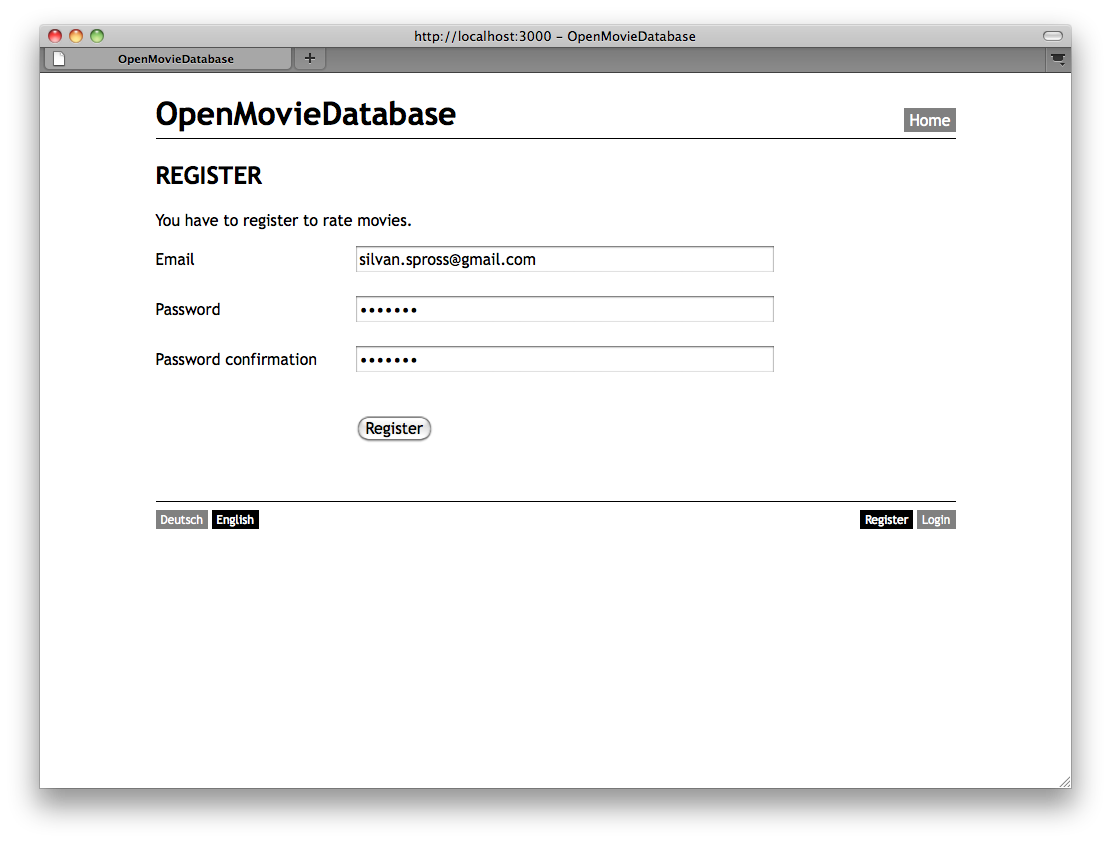
\includegraphics[width=0.9\textwidth,angle=0]{./bilder/tests/test_registrierung_01.png}
        \caption{Ausgefüllter Registrierungsscreen}
        \label{test_registrierung_01}
    \end{center}
\end{figure}

\begin{figure}[ht]
    \begin{center}
        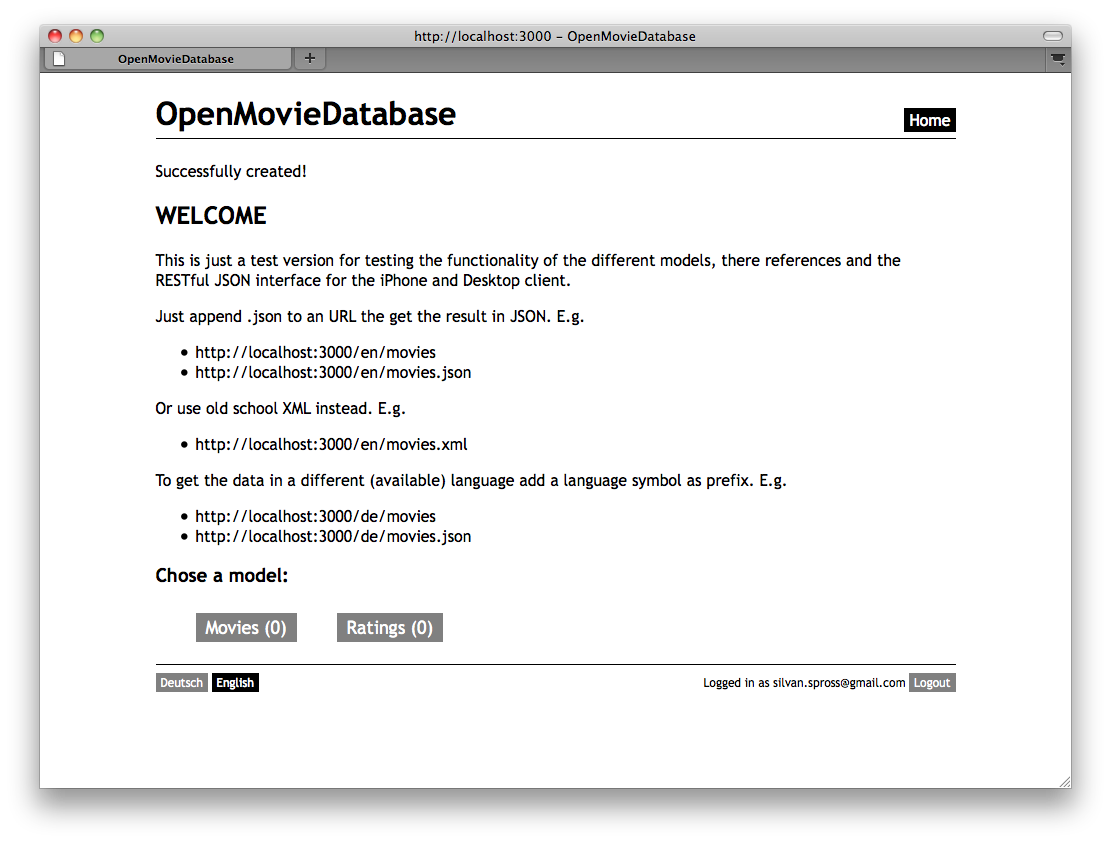
\includegraphics[width=0.9\textwidth,angle=0]{./bilder/tests/test_registrierung_02.png}
        \caption{Bestätigung der Registrierung}
        \label{test_registrierung_02}
    \end{center}
\end{figure}

Wie den Grafiken \ref{test_registrierung_01} und \ref{test_registrierung_02} zu 
entnehmen ist, hat die Registrierung funktioniert und ich versuche nun, mich 
nochmals mit dem selben Benutzernamen zu registrieren.

\begin{figure}[ht]
    \begin{center}
        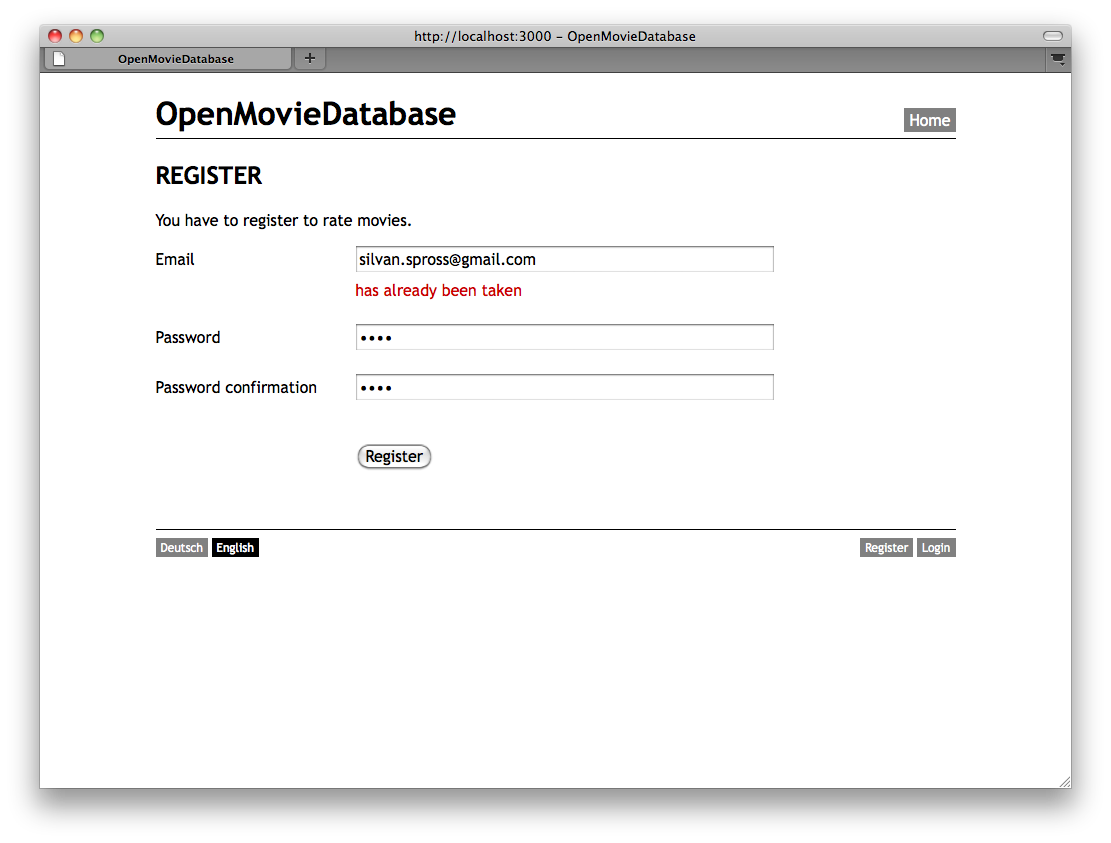
\includegraphics[width=0.9\textwidth,angle=0]{./bilder/tests/test_registrierung_03.png}
        \caption{Meldung, dass der Benutzername schon verwendet wird}
        \label{test_registrierung_03}
    \end{center}
\end{figure}

In der Grafik \ref{test_registrierung_03} werde ich darauf hingewiesen, dass
der Benutzername schon verwendet wurde.

\clearpage

\subsubsection{Anmeldung}
In der Grafik \ref{test_anmeldung_01} versuche ich mich nun mit meinem eben
registrierten Benutzer anzumelden.

\begin{figure}[ht]
    \begin{center}
        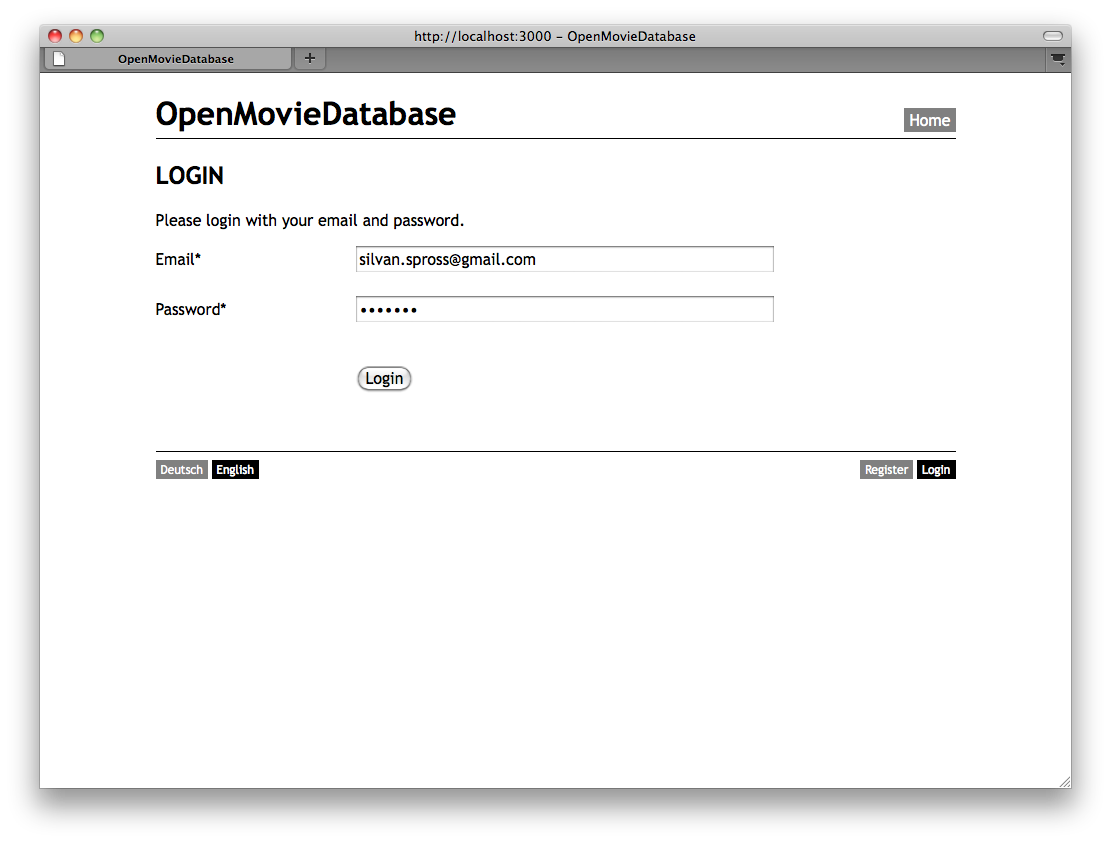
\includegraphics[width=0.9\textwidth,angle=0]{./bilder/tests/test_anmeldung_01.png}
        \caption{Ausgefüllter Anmeldescreen}
        \label{test_anmeldung_01}
    \end{center}
\end{figure}

Wie man der Grafik \ref{test_anmeldung_02} entnehmen kann, konnte ich mich
erfolgreich auf der Plattform anmelden. Dies ist zusätzlich erkennbar, da 
der Button unten rechts `Register' durch meinen Benutzernamen und der Button
`Login' durch den Button `Logout' ersetzt wurde.

\begin{figure}[ht]
    \begin{center}
        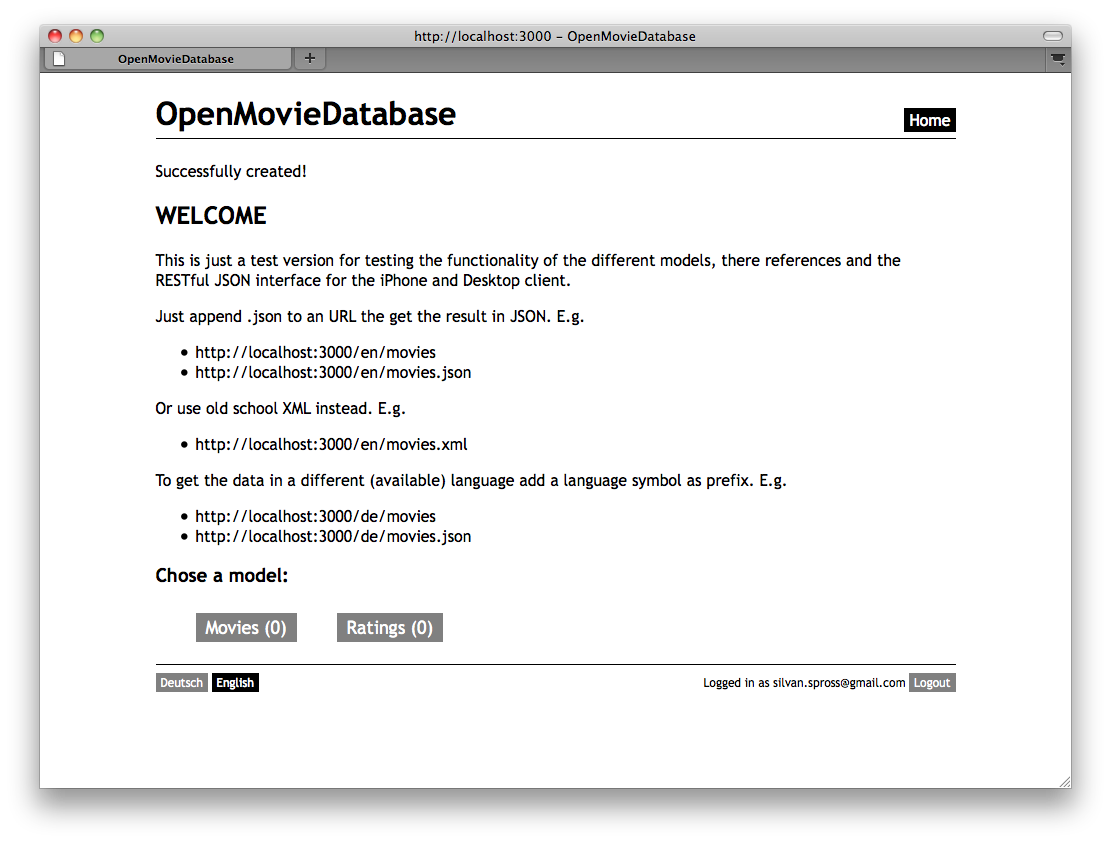
\includegraphics[width=0.9\textwidth,angle=0]{./bilder/tests/test_anmeldung_02.png}
        \caption{Homescreen nach der Anmeldung}
        \label{test_anmeldung_02}
    \end{center}
\end{figure}

\clearpage

\subsubsection{Filme verfassen}
Da auch Gäste Filme erfassen dürfen, melde ich mich wieder ab.
Jetzt versuche ich, wie in der Grafik \ref{test_movie_01} ersichtlich ist, einen neuen Film zu erfassen, 
indem ich den Filmerfassungsscreen aufrufe, ihn ausfülle und auf `Create Movie' klicke.

\begin{figure}[ht]
    \begin{center}
        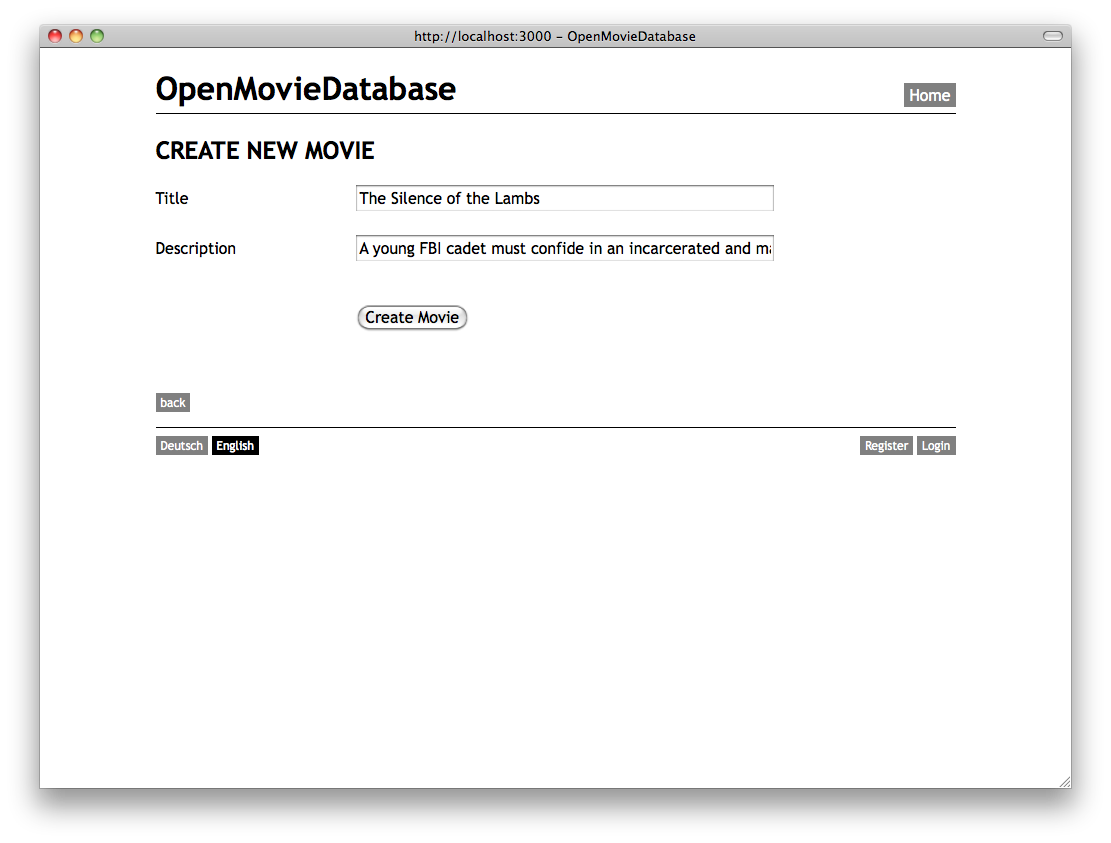
\includegraphics[width=0.9\textwidth,angle=0]{./bilder/tests/test_movie_01.png}
        \caption{Filmerfassungsscreen}
        \label{test_movie_01}
    \end{center}
\end{figure}

Auf der Grafik \ref{test_movie_02} sieht man, dass das Einfügen eines neuen
Filmes funktioniert hat. Ich sehe zudem, dass der Film bis jetzt noch nicht
bewertet wurde und dass ich mich anmelden müsste, um eine Bewertung abgeben zu
können.

\begin{figure}[ht]
    \begin{center}
        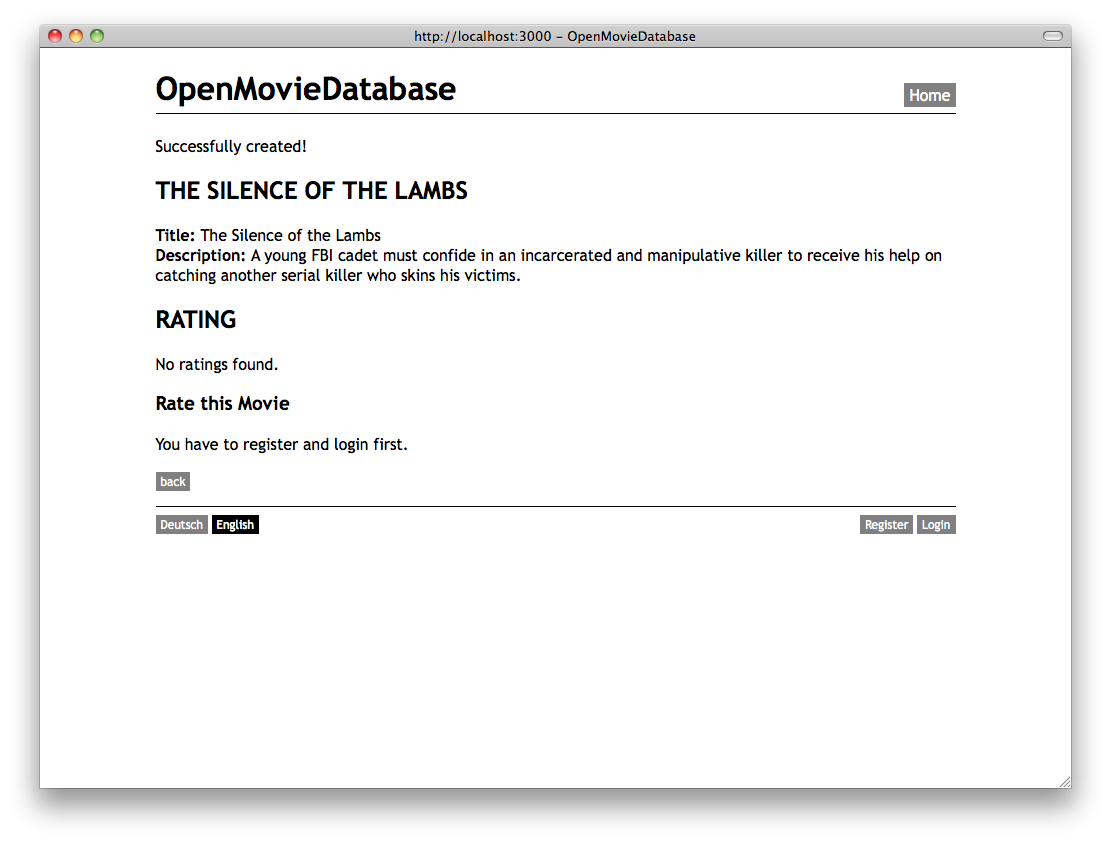
\includegraphics[width=0.9\textwidth,angle=0]{./bilder/tests/test_movie_02.png}
        \caption{Erfolgreich erfasster Film}
        \label{test_movie_02}
    \end{center}
\end{figure}

\clearpage

Jetzt werde ich versuchen, den Film zu bearbeiten. Dazu rufe ich den Bearbeitungsscreen
auf. In der Grafik \ref{test_movie_03} sieht man, dass die bestehend Informationen
schon abgefüllt sind. Ich passe die Beschreibung an und versuche den Film
zu speichern.

\begin{figure}[ht]
    \begin{center}
        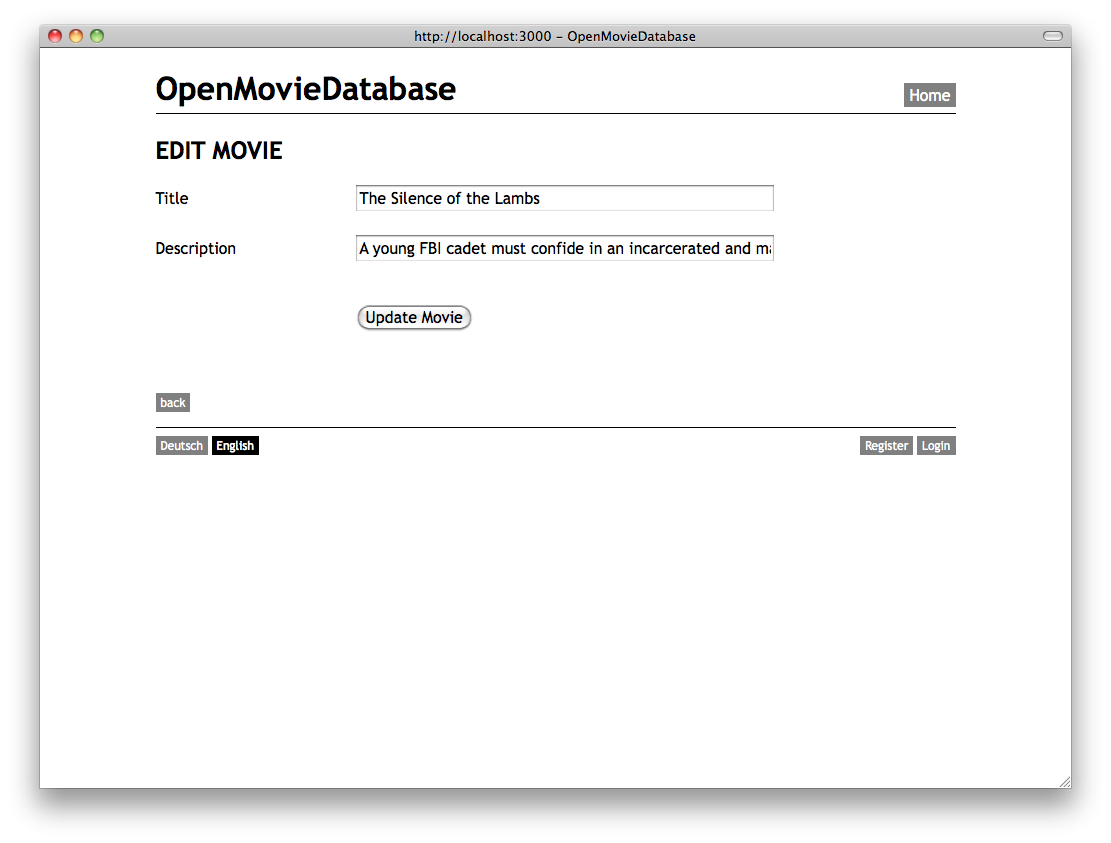
\includegraphics[width=0.9\textwidth,angle=0]{./bilder/tests/test_movie_03.png}
        \caption{Bearbeitungsscreen eines Filmes}
        \label{test_movie_03}
    \end{center}
\end{figure}

In der Grafik \ref{test_movie_04} sieht man, dass das bearbeiten des Filmes
funktioniert hat und nun in der Beschreibung der Name der Schauspielerin ergänzt
wurde.

\begin{figure}[ht]
    \begin{center}
        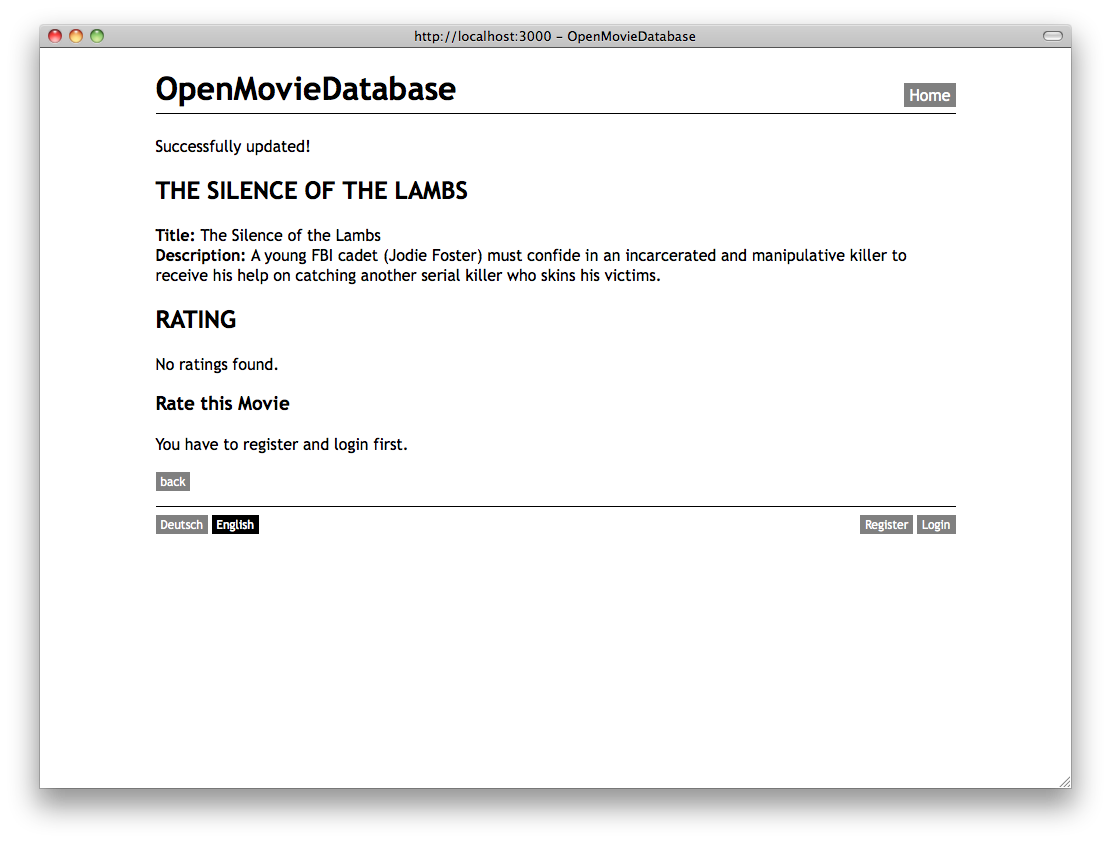
\includegraphics[width=0.9\textwidth,angle=0]{./bilder/tests/test_movie_04.png}
        \caption{Erfolgreich bearbeiteter Film}
        \label{test_movie_04}
    \end{center}
\end{figure}

\clearpage

Um zu testen, ob ein Film gelöscht werden kann, klicke ich in der Filmübersicht
beim existierenden Film auf `delete'. Dies sieht man auf der Grafik \ref{test_movie_05}.

\begin{figure}[ht]
    \begin{center}
        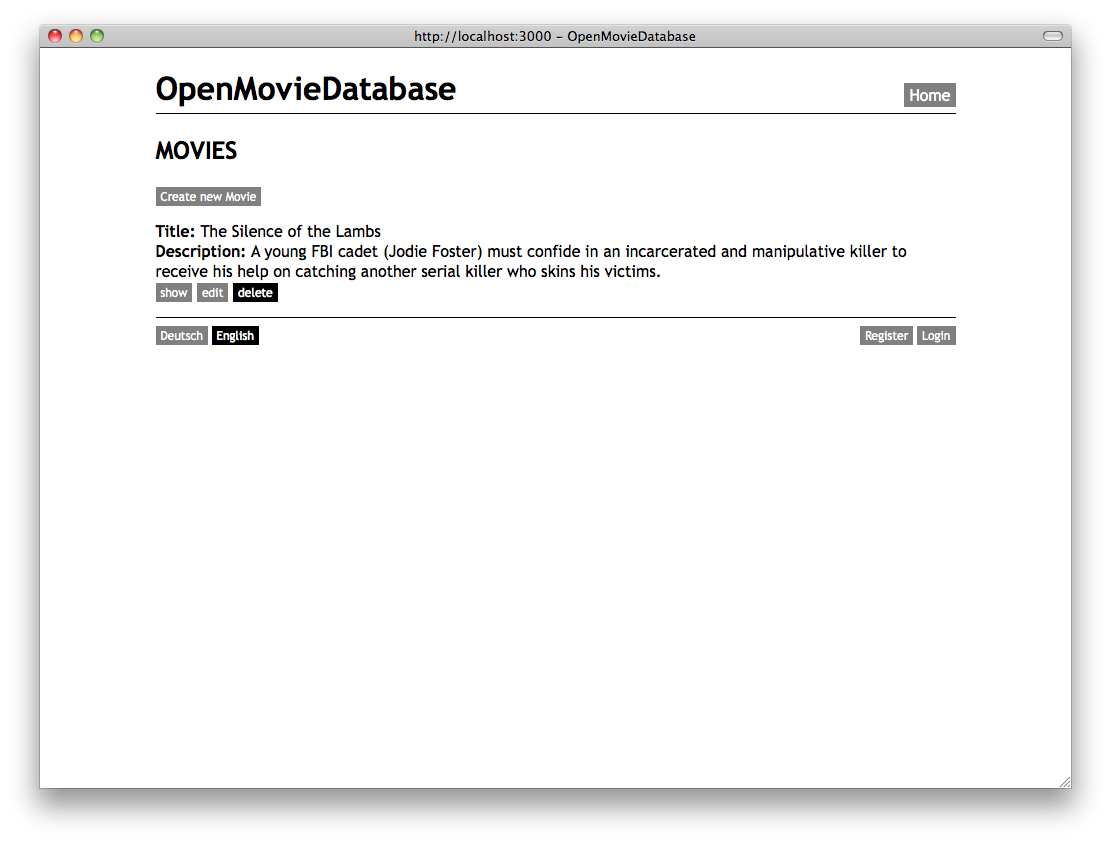
\includegraphics[width=0.9\textwidth,angle=0]{./bilder/tests/test_movie_05.png}
        \caption{Filmübersicht}
        \label{test_movie_05}
    \end{center}
\end{figure}

Wie man der Grafik \ref{test_movie_06} entnehmen kann, sieht man nach dem Löschen
die Meldung, dass der Film erfolgreich gelöscht wurde. Die Liste in der
Filmübersicht ist jetzt wieder leer.

\begin{figure}[ht]
    \begin{center}
        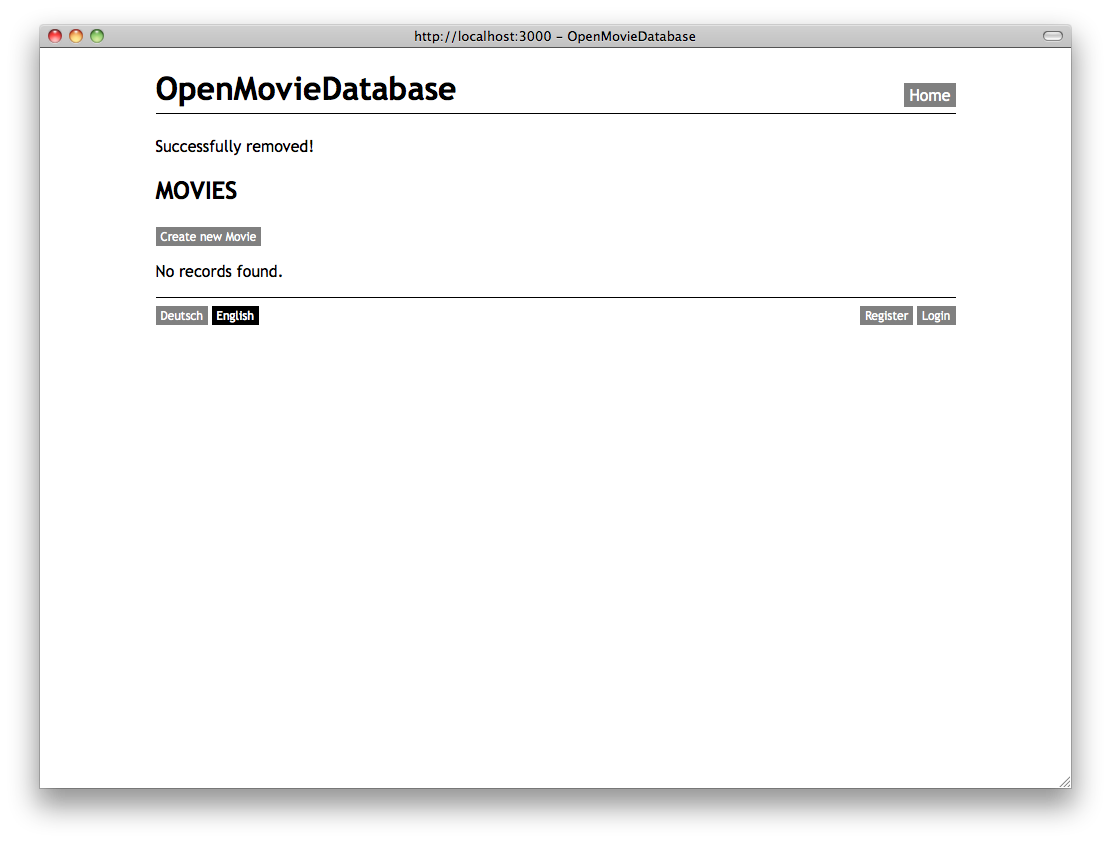
\includegraphics[width=0.9\textwidth,angle=0]{./bilder/tests/test_movie_06.png}
        \caption{Erfolgreich gelöschter Film}
        \label{test_movie_06}
    \end{center}
\end{figure}

\clearpage

\subsubsection{Bewertung abgeben}
Ich erfasse den soeben entfernten Film erneut und erfasse zusätzlich zwei Benutzer
`Stefan' und `Roman'. Ich gebe mit allen Benutzern eine Bewertung ab. In der Grafik
\ref{test_bewertung_01} sieht man die Maske zur Abgabe einer Bewertung, sofern man
angemeldet ist.

\begin{figure}[ht]
    \begin{center}
        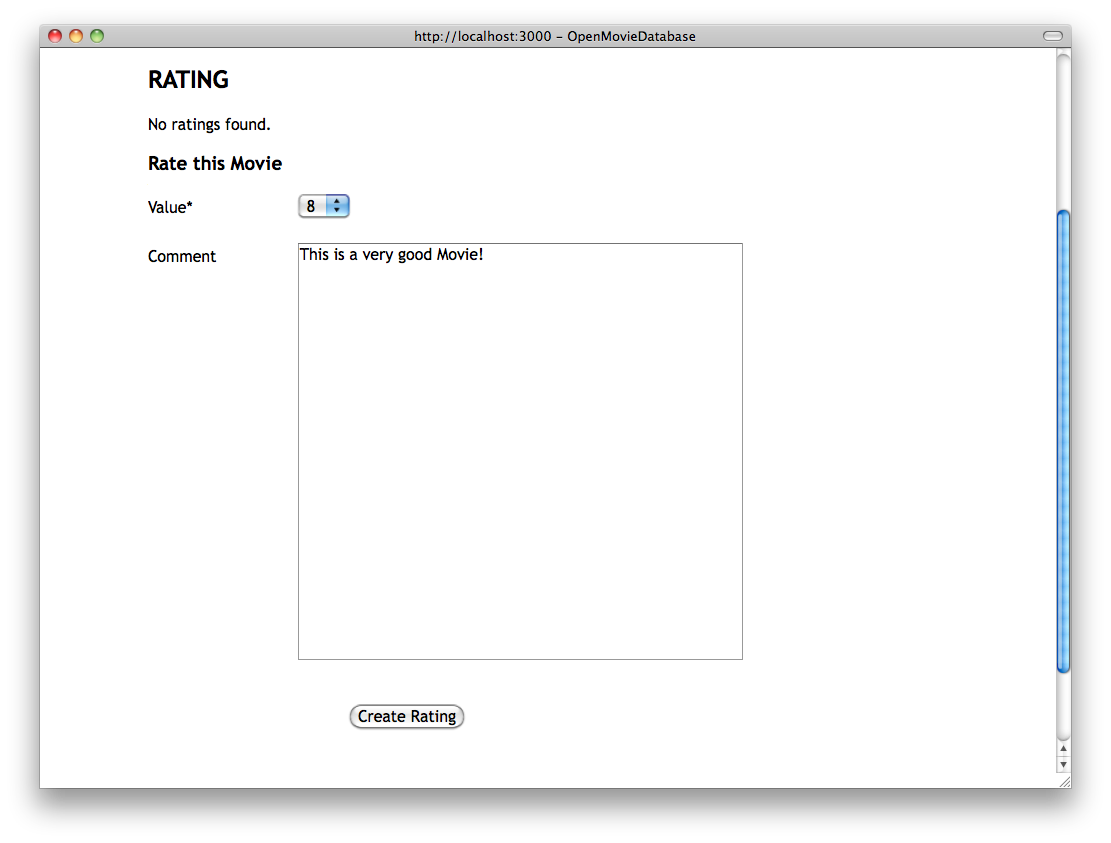
\includegraphics[width=0.9\textwidth,angle=0]{./bilder/tests/test_bewertung_01.png}
        \caption{Maske zur Erfassung einer Bewertung}
        \label{test_bewertung_01}
    \end{center}
\end{figure}

Sobald man die Bewertung abgegeben hat, erscheint, wie auf der Grafik \ref{test_bewertung_02}
zu sehen ist, die Detailansicht des Filmes erneut, jedoch nun mit einer Bewertung
und dem Hinweis, dass ich bereits eine Bewertung abgegeben habe.

\begin{figure}[ht]
    \begin{center}
        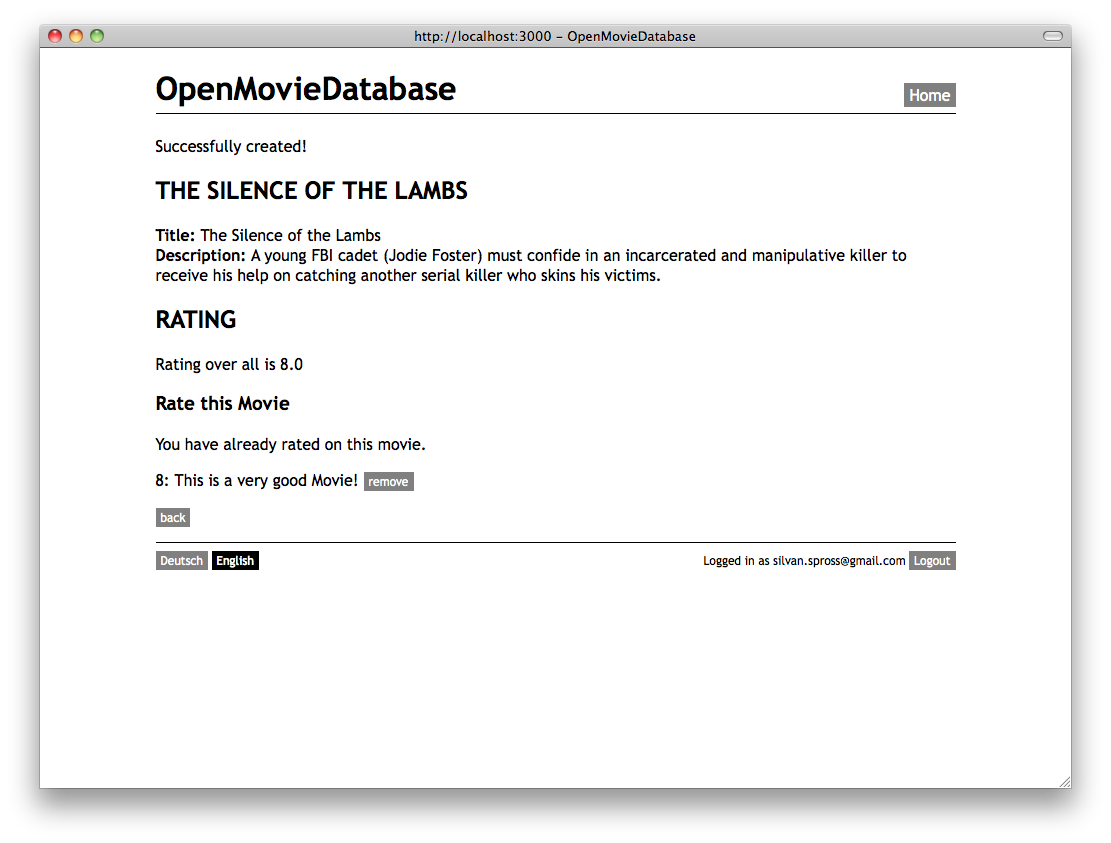
\includegraphics[width=0.9\textwidth,angle=0]{./bilder/tests/test_bewertung_02.png}
        \caption{Erfolgreich erfasste Bewertung}
        \label{test_bewertung_02}
    \end{center}
\end{figure}

\clearpage

\subsubsection{Bewertung sehen}
Ich melde mich von der Plattform ab um zu überprüfen, ob Gäste die Bewertung
des Filmes auch sehen können. Dies funktioniert und ist in der Grafik \ref{test_bewertung_03}
zu sehen. Unten rechts kann man am `Login' Button erkennen, dass zur Zeit
kein Benutzer angemeldet ist.

\begin{figure}[ht]
    \begin{center}
        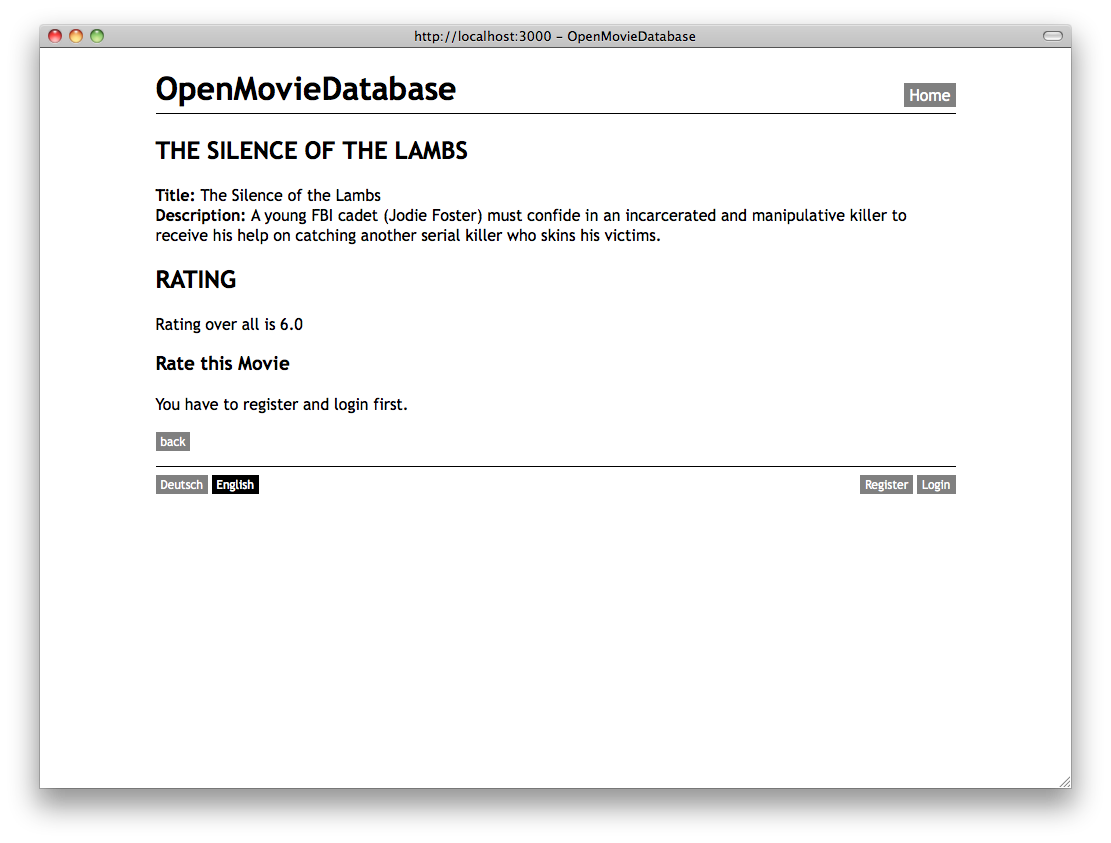
\includegraphics[width=0.9\textwidth,angle=0]{./bilder/tests/test_bewertung_03.png}
        \caption{Bewertungsansicht für Gäste}
        \label{test_bewertung_03}
    \end{center}
\end{figure}

\subsubsection{Bewertung Freundeskreis}
Damit ich die Bewertungsfunktionen richtig testen kann, schliesse ich
zwischen meinem Benutzer und dem Benutzer `Stefan' Freundschaft. Danach sollten 
die zwei befreundeten Benutzer ein zusätzliches Rating sehen, welches der dritte 
Benutzer nicht sieht. 

Wie man der Grafik \ref{test_bewertung_04} entnehmen kann, sieht der Benutzer
`Roman' nur die Bewertung über alle Benutzer und seine eigene. In der Grafik
\ref{test_bewertung_05} ist zu sehen, dass mein Benutzer zusätzlich eine
Bewertung seines Freundeskreises sieht.

\begin{figure}[ht]
    \begin{center}
        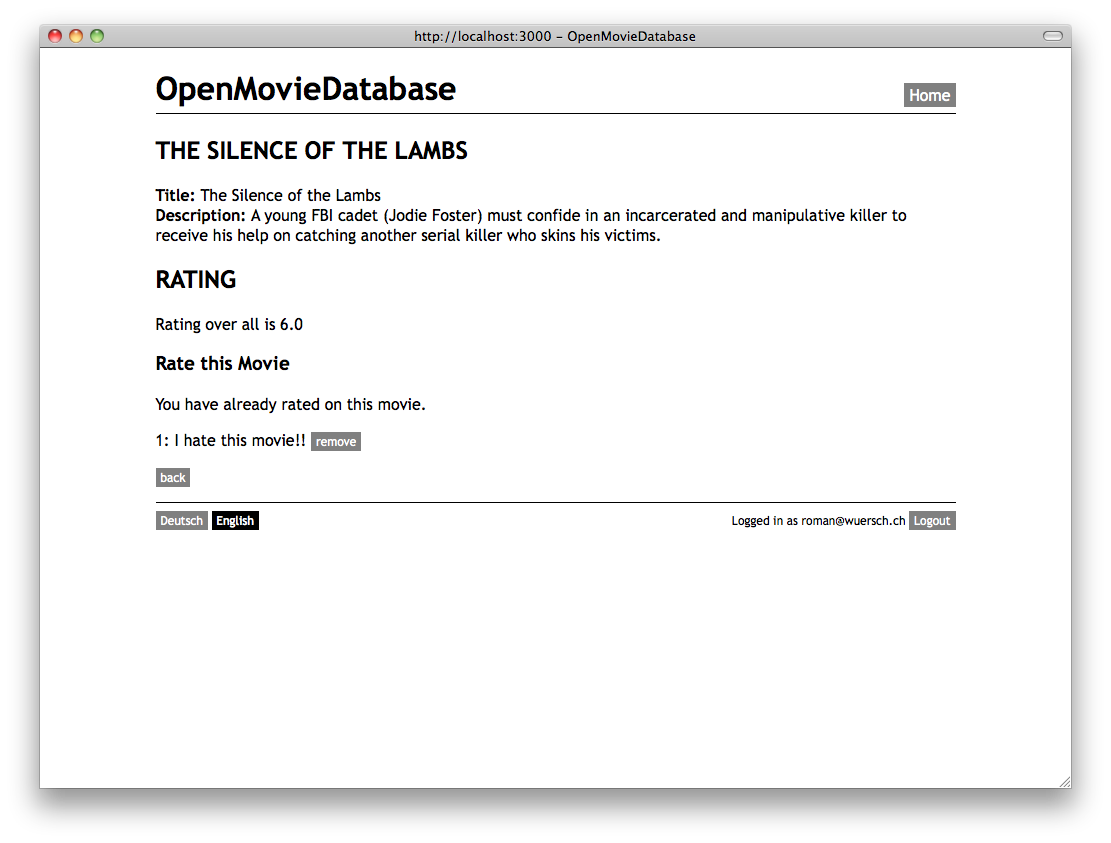
\includegraphics[width=0.9\textwidth,angle=0]{./bilder/tests/test_bewertung_04.png}
        \caption{Ansicht des Benutzers `Roman'}
        \label{test_bewertung_04}
    \end{center}
\end{figure}

\begin{figure}[ht]
    \begin{center}
        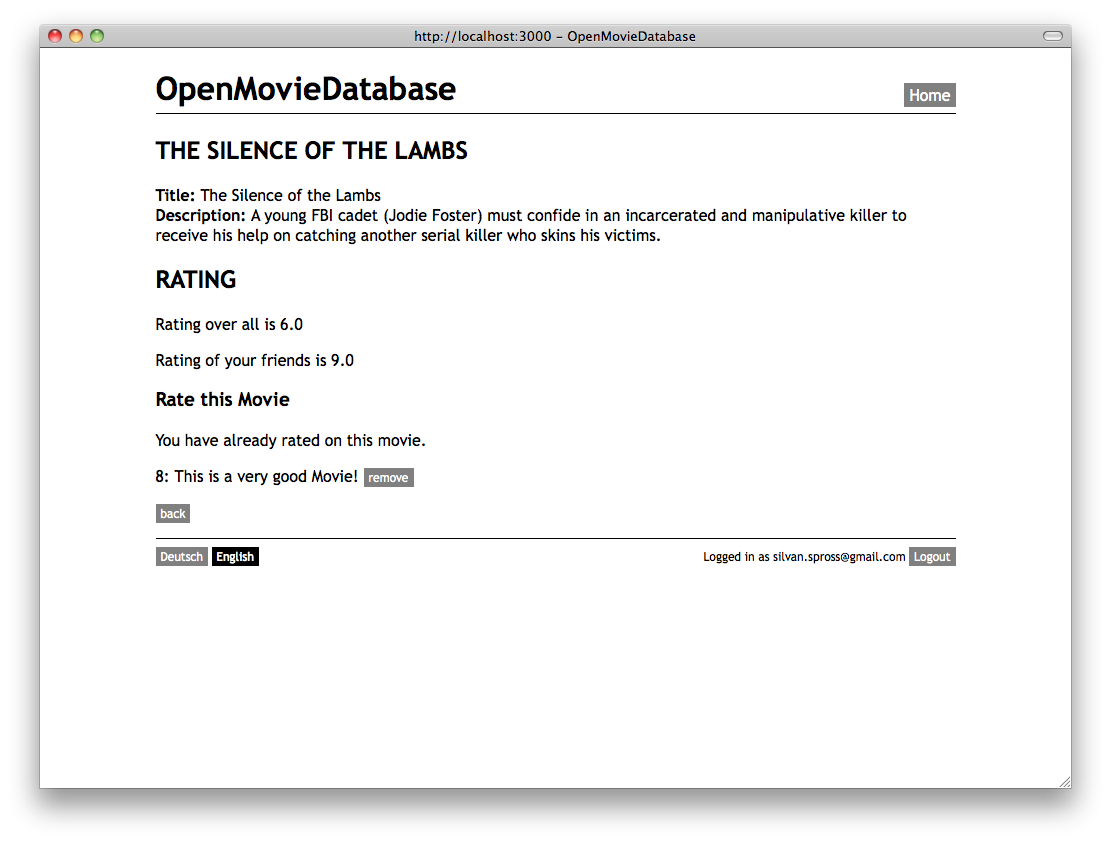
\includegraphics[width=0.9\textwidth,angle=0]{./bilder/tests/test_bewertung_05.png}
        \caption{Ansicht meines Benutzers}
        \label{test_bewertung_05}
    \end{center}
\end{figure}

\clearpage

\subsubsection{Internationalisierung}
Ich habe die Plattform für die Sprachen ``Deutsch'' und ``Englisch'' vorbereitet.
Das bedeutet, alle statischen Texte dieser Sprachen sind im Quellcode hinterlegt.

Die dynamischen Texte, also zum Beispiel der Name und die Beschreibung eines
Filmes, müssen in beiden Sprachen erfasst werden. Dazu ruft man den Bearbeitungsscreen
eines bestehenden Filmes auf und wechselt unten links die Sprache der Plattform.
Wenn nun der neue Inhalt in der aktuellen Sprache erfasst wird, wird dieser 
zusätzlich zum Film abgelegt. Ich werde den deutschen Inhalt des bestehendes Filmes 
auf diese Weise nun erfassen.

In der Grafik \ref{test_internationalisierung_01} sieht man den bestehenden Film,
während die Plattform in der Sprache ``Englisch'' dargestellt wird. Dies kann man
unten links an der gewählten Sprache erkennen. In der Grafik \ref{test_internationalisierung_02}
ist die Sprache auf ``Deutsch'' gewählt und der Inhalt, wie auch die statischen 
Texte werden in ``Deutsch'' dargestellt.

\begin{figure}[ht]
    \begin{center}
        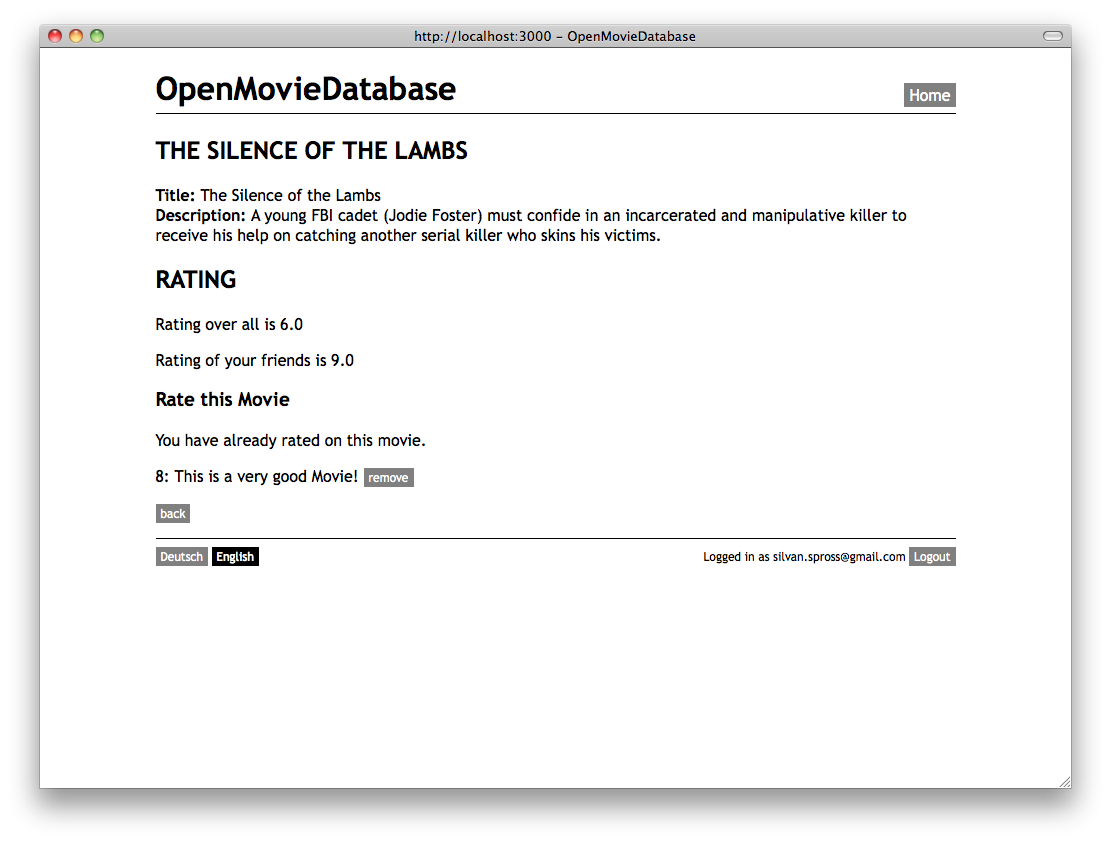
\includegraphics[width=0.9\textwidth,angle=0]{./bilder/tests/test_internationalisierung_01.png}
        \caption{Filmansicht in ``Englisch''}
        \label{test_internationalisierung_01}
    \end{center}
\end{figure}

\begin{figure}[ht]
    \begin{center}
        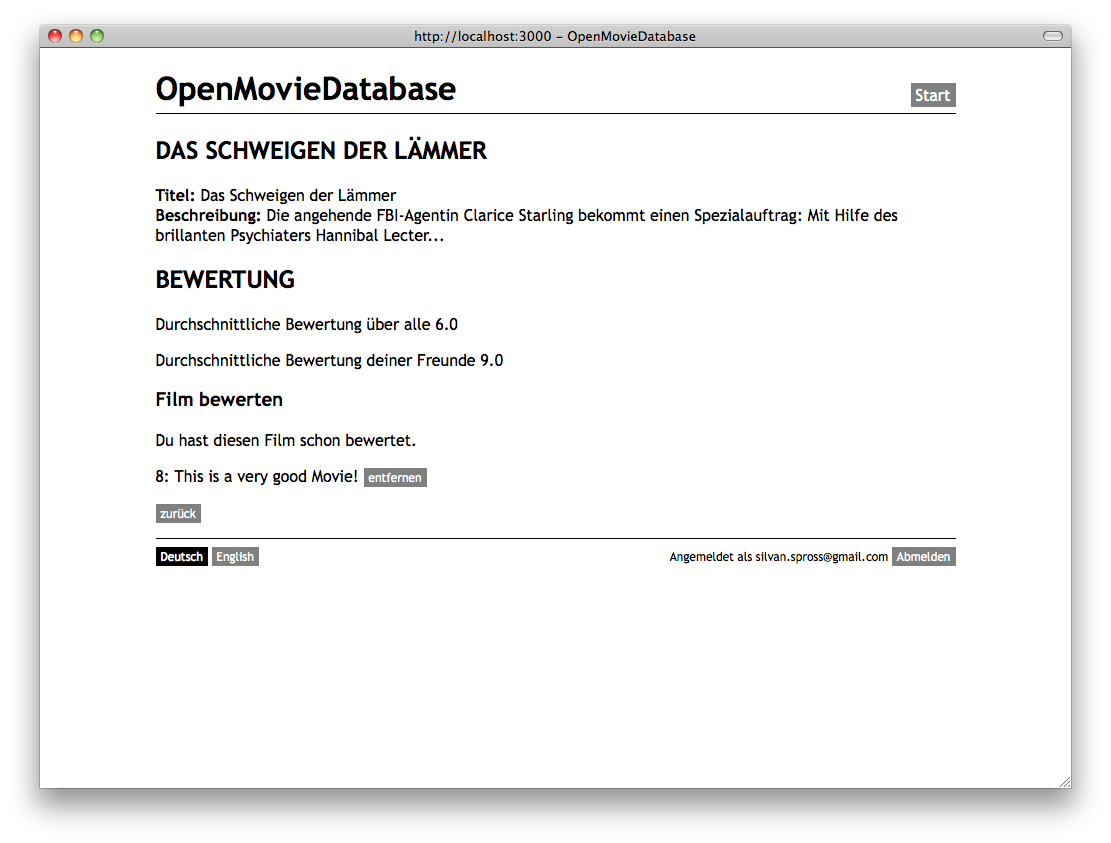
\includegraphics[width=0.9\textwidth,angle=0]{./bilder/tests/test_internationalisierung_02.png}
        \caption{Filmansicht in ``Deutsch''}
        \label{test_internationalisierung_02}
    \end{center}
\end{figure}

\clearpage

\subsubsection{Schnittstelle}
Um die API zu testen, verwende ich absichtlich ein Programm, das in einer
anderen Sprache als `Ruby' geschrieben ist. Das Programm, das ich verwende
heisst ``RESTClient'', ist in `Java' geschrieben und ist unter 
\url{http://code.google.com/p/rest-client/} verfügbar. Ich verwende es in der 
Version 2.3. Zusätzlich ist zu erwähnen, dass die Daten in beiden verfügbaren
Sprachen bezogen werden könne. Dies wird über die URL gesteuert. 

Wie man in der Grafik \ref{test_schnittstelle_01} erkennen kann, wird ein
sauberes XML zurückgeliefert, wenn man die Filme über einen `HTTP GET' beziehen 
möchte. Auch sieht man, dass das Rating ebenfalls mitgeliefert wird.

\begin{figure}[ht]
    \begin{center}
        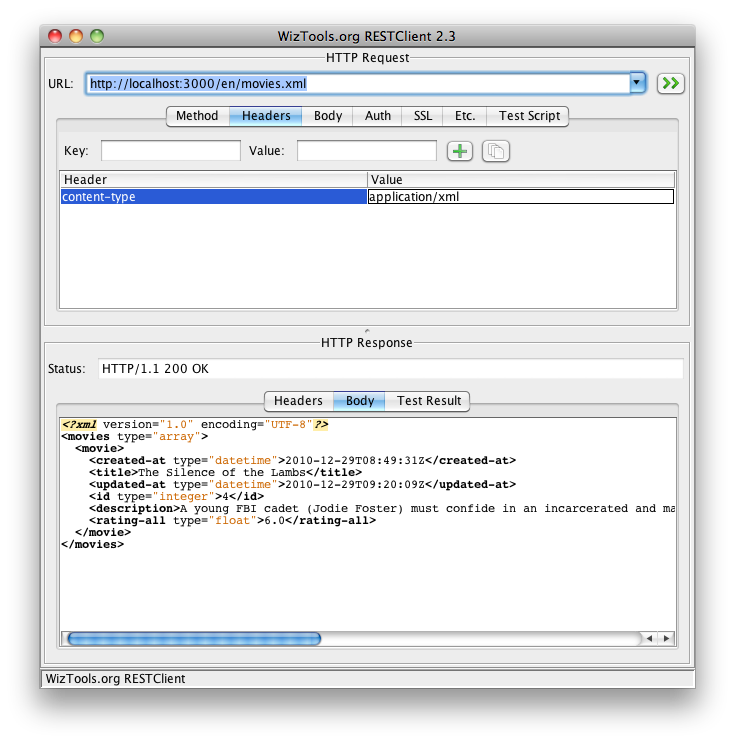
\includegraphics[width=0.9\textwidth,angle=0]{./bilder/tests/test_schnittstelle_01.png}
        \caption{API `HTTP GET' der Filme}
        \label{test_schnittstelle_01}
    \end{center}
\end{figure}

In der Grafik \ref{test_schnittstelle_02} sieht man, dass auch ein einzelner
Film abgerufen werden kann.

\begin{figure}[ht]
    \begin{center}
        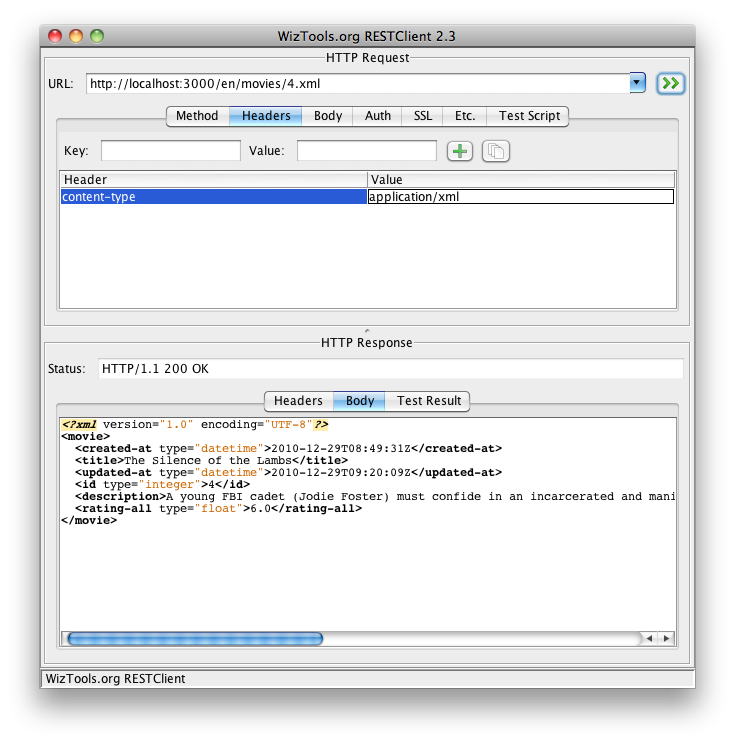
\includegraphics[width=0.9\textwidth,angle=0]{./bilder/tests/test_schnittstelle_02.png}
        \caption{API `HTTP GET' eines Filmes}
        \label{test_schnittstelle_02}
    \end{center}
\end{figure}

\clearpage

Auch kann ein neuer Film über einen `HTTP POST' erstellt werden, dies sieht man
in den Grafiken \ref{test_schnittstelle_03} und \ref{test_schnittstelle_04},
in welchen der Film dann in der Filmübersicht ersichtlich ist.

\begin{figure}[ht]
    \begin{center}
        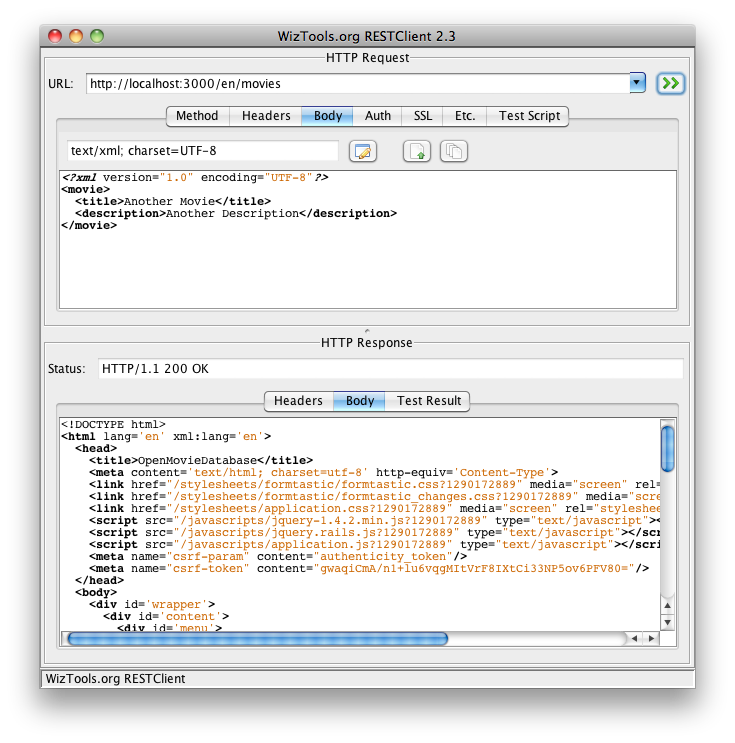
\includegraphics[width=0.9\textwidth,angle=0]{./bilder/tests/test_schnittstelle_03.png}
        \caption{API `HTTP POST' eines Filmes}
        \label{test_schnittstelle_03}
    \end{center}
\end{figure}

\begin{figure}[ht]
    \begin{center}
        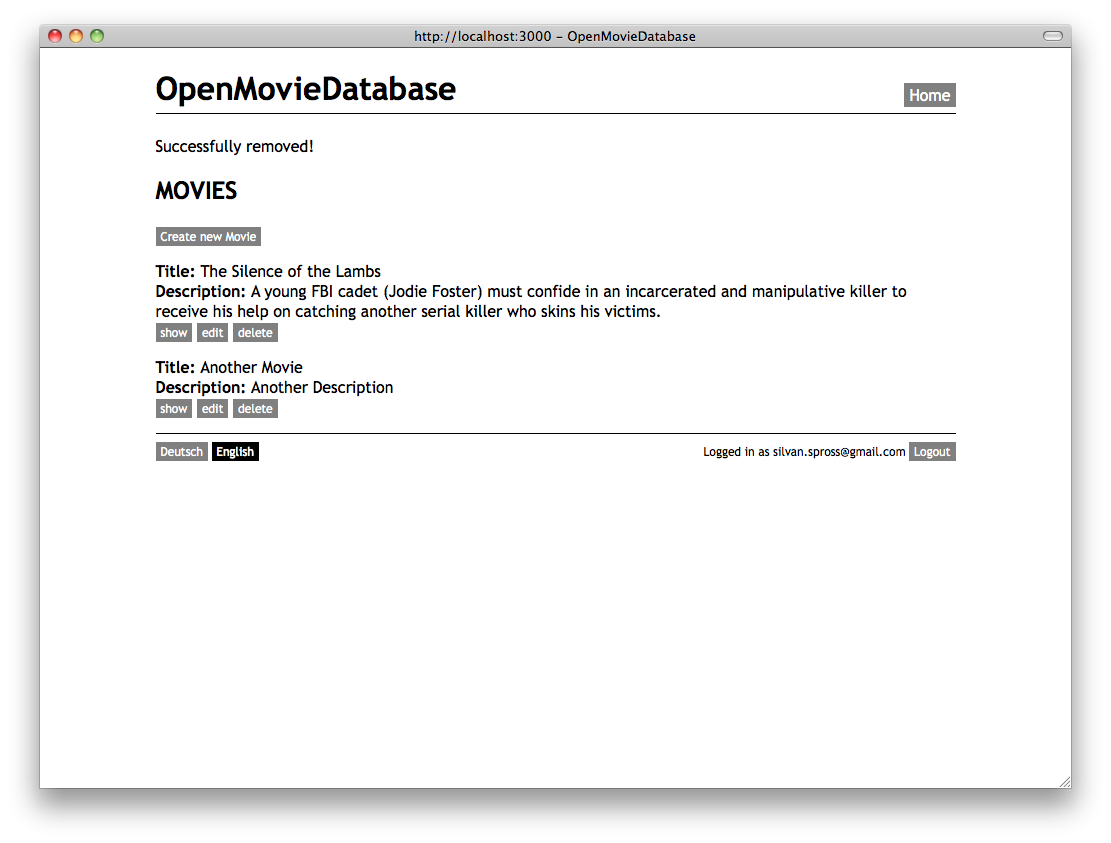
\includegraphics[width=0.9\textwidth,angle=0]{./bilder/tests/test_schnittstelle_04.png}
        \caption{Filmübersicht mit über die API eingefügtem Film}
        \label{test_schnittstelle_04}
    \end{center}
\end{figure}

\clearpage

Der eingefügte Film kann auch wieder über einen `HTTP PUT' bearbeitet werden,
was in den Grafiken \ref{test_schnittstelle_05} und \ref{test_schnittstelle_06}
zu erkennen ist.

\begin{figure}[ht]
    \begin{center}
        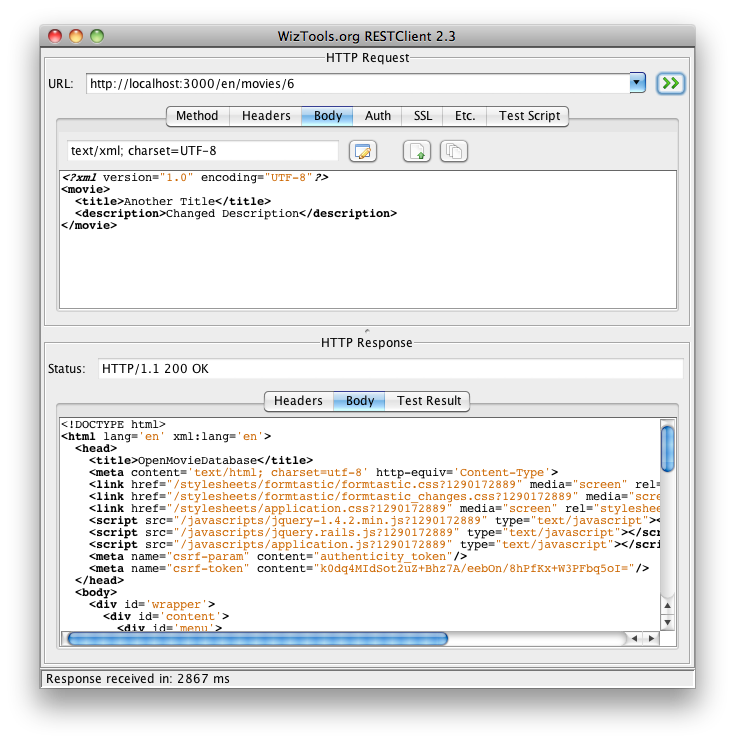
\includegraphics[width=0.9\textwidth,angle=0]{./bilder/tests/test_schnittstelle_05.png}
        \caption{API `HTTP PUT' eines Filmes}
        \label{test_schnittstelle_05}
    \end{center}
\end{figure}

\begin{figure}[ht]
    \begin{center}
        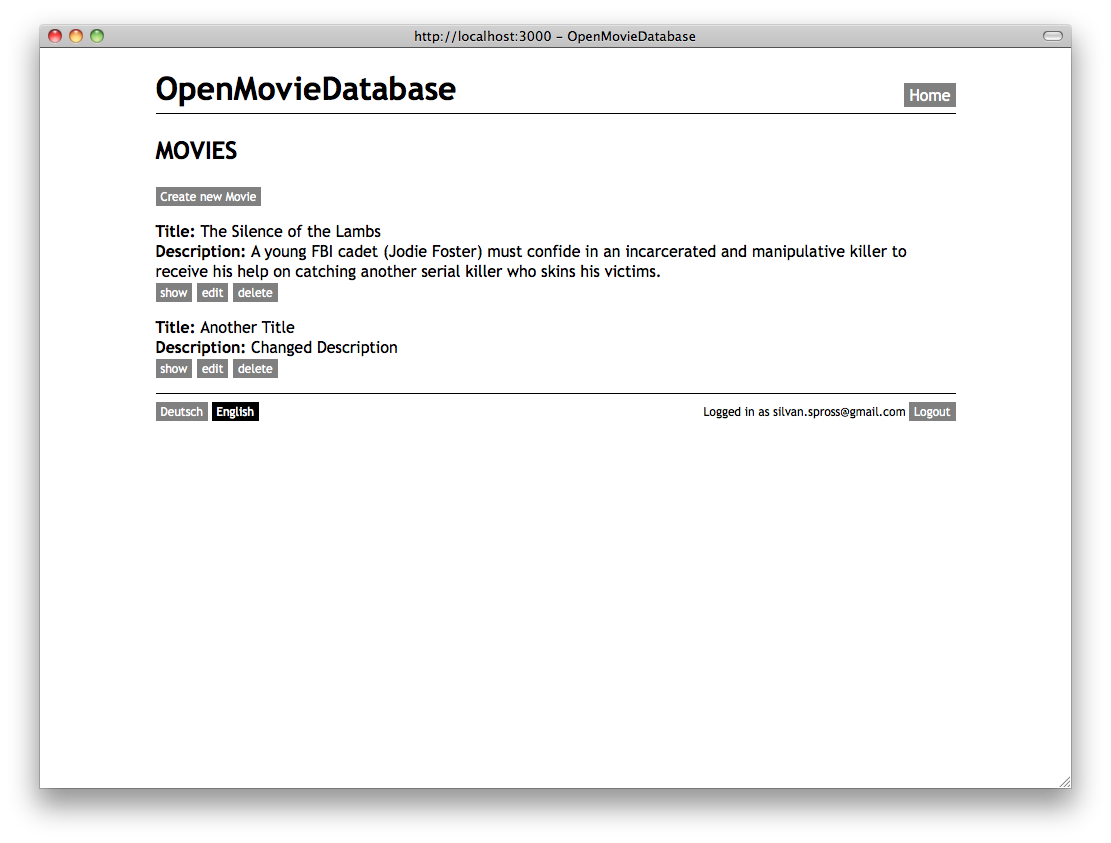
\includegraphics[width=0.9\textwidth,angle=0]{./bilder/tests/test_schnittstelle_06.png}
        \caption{Filmübersicht mit über die API geändertem Film}
        \label{test_schnittstelle_06}
    \end{center}
\end{figure}

\clearpage

Auch kann ein Film über einen `HTTP DELETE' gelöscht werden. Ich verzichte
hier auf zusätzliche Grafiken, da sie nicht viel Aussagekraft haben.

\subsection{Testresultate}
In der nachstehenden Tabelle \ref{tab:testresultate} gehe ich noch einmal
durch meine in der Tabelle \ref{tab:testfaelle} definierten Testfälle
und ergänze, ob sie erfolgreich waren oder nicht.

\begin{table}[ht]
\begin{center}
    \begin{tabular}{llc}
        \toprule Nr & Muss-Funktions Nr & Erfolgreich \\
        \midrule 1 & 1 & ja \\
        \midrule 2 & 1 & ja \\
        \midrule 3 & 2 & ja \\
        \midrule 4 & 3 & ja \\
        \midrule 5 & 3 & ja \\
        \midrule 6 & 3 & ja \\
        \midrule 7 & 4 & ja \\
        \midrule 8 & 5 & ja \\
        \midrule 9 & 6 & ja \\
        \midrule 10 & 7 & ja \\
        \midrule 11 & 8 & ja \\
        \midrule 12 & 8 & ja \\
        \midrule 13 & 8 & ja \\
        \midrule 14 & 8 & ja \\
        \bottomrule
    \end{tabular}
    \caption{Testresultate}
    \label{tab:testresultate}
\end{center}
\end{table}

Somit sind alle meine Muss-Funktionen erfüllt und ich habe mein Ziel erreicht.
Zusätzlich zu den Testresultaten habe ich noch einen Screenshot meiner
Unit-Test Ergebnisse zum Zeitpunkt der Abgabe der Arbeit als Grafik \ref{unit_testresultate}
beigefügt.

\begin{figure}[ht]
    \begin{center}
        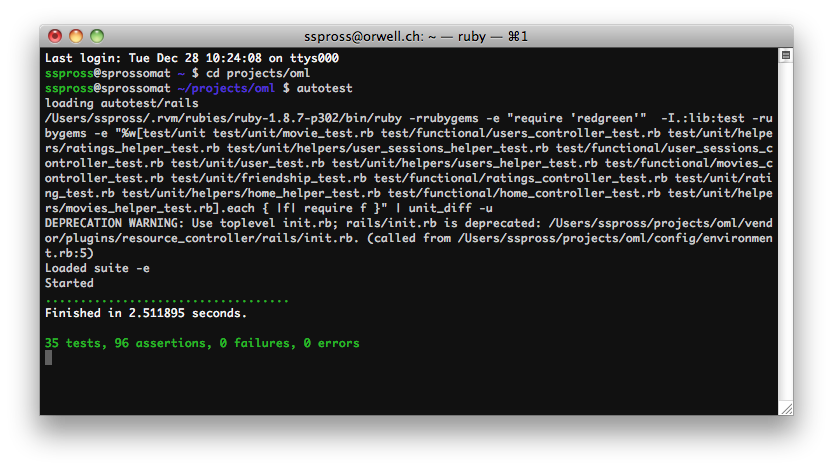
\includegraphics[width=0.9\textwidth,angle=0]{./bilder/testresultate.png}
        \caption{Testresultat vom 28.12.2010}
        \label{unit_testresultate}
    \end{center}
\end{figure}